\documentclass[border=20pt, tikz]{standalone}
\usepackage{amsmath}
\usetikzlibrary{calc, arrows.meta, decorations.pathreplacing}

% =========================================================
% GLOBAL SETTINGS
% =========================================================
\tikzset{
    glass/.style={fill=cyan!15, draw=cyan!70!blue, thick, fill opacity=0.2, line join=round},
    ray/.style={draw=orange, thick, -{Latex[length=1.5mm]}},
    axis/.style={thick, -{Latex[length=3mm, width=2mm]}},
    common settings/.style={
        font=\sffamily\small,
        x={(0.9cm, -0.15cm)}, 
        y={(0cm, 1cm)}, 
        z={(-0.6cm, -0.5cm)}
    }
}

\begin{document}

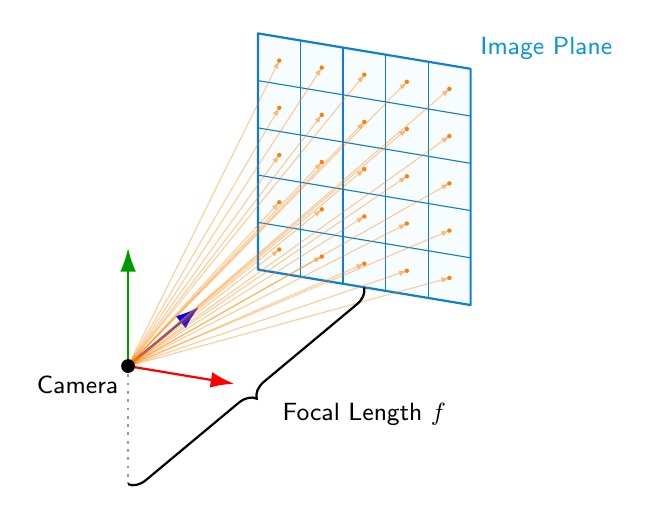
\begin{tikzpicture}[common settings]

    % Configuration
    \def\zdist{5}      % Distance of image plane from camera
    \def\res{5}        % 5x5 resolution
    \def\pixSize{0.6}  % Size of each pixel
    \pgfmathsetmacro{\halfW}{(\res * \pixSize) / 2}

    % 1. Draw World Axes
    \draw[axis, red] (0,0,0) -- (1.5,0,0);
    \draw[axis, green!60!black] (0,0,0) -- (0,1.5,0);
    \draw[axis, blue] (0,0,0) -- (0,0,-1.5);
    
    % 2. Draw Image Plane (Glass)
    \path[glass] (-\halfW, -\halfW, -\zdist) -- (\halfW, -\halfW, -\zdist) 
              -- (\halfW, \halfW, -\zdist) -- (-\halfW, \halfW, -\zdist) -- cycle;

    % 3. Draw 5x5 Grid Lines
    \foreach \i in {0,...,\res} {
        \pgfmathsetmacro{\pos}{-\halfW + \i * \pixSize}
        % Vertical lines
        \draw[cyan!60!blue, thin] (\pos, -\halfW, -\zdist) -- (\pos, \halfW, -\zdist);
        % Horizontal lines
        \draw[cyan!60!blue, thin] (-\halfW, \pos, -\zdist) -- (\halfW, \pos, -\zdist);
    }

    % 4. Generate Rays to Pixel Centers
    % We iterate 0 to 4 for a 5x5 grid
    % 4. Generate Rays to Pixel Centers
    \foreach \ix in {0,...,4} {
        \foreach \iy in {0,...,4} {
            % Calculate pixel center coordinate
            \pgfmathsetmacro{\px}{-\halfW + (\ix + 0.5) * \pixSize}
            \pgfmathsetmacro{\py}{-\halfW + (\iy + 0.5) * \pixSize}
            
            % Added -{Latex[length=1mm]} to the options below
            \draw[orange, opacity=0.4, line width=0.4pt, -{Latex[length=1mm]}] (0,0,0) -- (\px, \py, -\zdist);
            
            % Draw a small dot at the pixel center
            \fill[orange] (\px, \py, -\zdist) circle (0.8pt);
        }
    }

    % 5. Highlight one specific "Primary Ray" for labeling
    % \pgfmathsetmacro{\targetX}{-\halfW + (3 + 0.5) * \pixSize}
    % \pgfmathsetmacro{\targetY}{-\halfW + (3 + 0.5) * \pixSize}
    % \draw[ray, orange, line width=1.2pt] (0,0,0) -- (\targetX, \targetY, -\zdist);
    
    % 6. Labels and Annotations
    \fill[black] (0,0,0) circle (2.5pt) node[below left] {Camera};
    
    % \node[orange, right] at (\targetX, \targetY, -\zdist) {$\mathbf{d}_{ij}$};
    \node[cyan!80!blue, anchor=south west] at (\halfW, \halfW, -\zdist) {Image Plane};
    
    % Focal length brace
    \draw[decorate, decoration={brace, amplitude=6pt, mirror}, thick]
        (0, -1.5, 0) -- (0, -1.5, -\zdist) 
        node[below, below=38pt] {Focal Length $f$};

    \draw[black, opacity=0.4, line width=1pt, dotted] (0,0,0) -- (0, -1.5, 0);

    

\end{tikzpicture}

\end{document}